\section{Persistenz}

\begin{concept}{Persistenz Grundlagen}\\
Persistenz bezeichnet die dauerhafte Speicherung von Daten über das Programmende hinaus:
\begin{itemize}
    \item Speicherung in Datenbankmanagementsystemen (DBMS)
    \item Haupttypen:
    \begin{itemize}
        \item Relationale Datenbanksysteme (RDBMS)
        \item NoSQL-Datenbanken (ohne fixes Schema)
    \end{itemize}
    \item O/R-Mapping (Object Relational Mapping)
    \begin{itemize}
        \item Abbildung zwischen Objekten und Datensätzen
        \item Überwindung des Strukturbruchs (Impedance Mismatch)
    \end{itemize}
\end{itemize}
\end{concept}

\begin{KR}{Best Practices für Persistenz}

    \begin{minipage}[t]{0.5\textwidth}
\textbf{1. Architektur-Ebene}
\begin{itemize}
    \item Trennung von Concerns
    \begin{itemize}
        \item Repository für Datenzugriff
        \item Service für Geschäftslogik
        \item DTO für Datentransfer
    \end{itemize}
    \item Transaktionsmanagement
    \begin{itemize}
        \item Auf Service-Ebene
        \item Atomare Operationen
        \item Konsistente Daten
    \end{itemize}
\end{itemize}
\end{minipage}
\begin{minipage}[t]{0.5\textwidth}
\textbf{2. Entity Design}
\begin{itemize}
    \item Immutable wenn möglich
    \item Validierung durch\\ Bean Validation
    \item Geschäftsregeln in\\ Entity-Klassen
\end{itemize}

\textbf{3. Performance Optimierung}
\begin{itemize}
    \item Caching Strategien
    \item Batch Processing
    \item Query Optimierung
\end{itemize}
\end{minipage}
\end{KR}

\begin{definition}{O/R-Mismatch}\\
Der Strukturbruch zwischen objektorientierter und relationaler Welt:
\begin{itemize}
    \item \textbf{Typen-Systeme:}
    \begin{itemize}
        \item Unterschiedliche NULL-Behandlung
        \item Datum/Zeit-Darstellung
    \end{itemize}
    \item \textbf{Beziehungen:}
    \begin{itemize}
        \item Richtung der Beziehungen
        \item Mehrfachbeziehungen
        \item Vererbung
    \end{itemize}
    \item \textbf{Identität:}
    \begin{itemize}
        \item OO: Implizite Objektidentität
        \item DB: Explizite Identität (Primary Key)
    \end{itemize}
    \item \textbf{Besondere Herausforderungen:}
    \begin{itemize}
        \item Unterschiedliche Repräsentationsformen
        \item Flache Tabellenstruktur vs. Objekthierarchien
        \item Verschiedene Konzepte für Beziehungen
    \end{itemize}
\end{itemize}
\end{definition}



\begin{example2}{Prüfungsaufgabe: O/R-Mapping Analyse}\\
\textbf{Szenario:}
Ein Universitätssystem verwaltet Studenten, Kurse und Noten. Studenten können mehrere 
Kurse belegen, ein Kurs hat mehrere Studenten.

\textbf{Aufgabe:} 
Analysieren Sie die O/R-Mapping Herausforderungen dieser Domain.

\textbf{Lösung:}
\begin{itemize}
    \item \textbf{Beziehungen:}
    \begin{itemize}
        \item Many-to-Many zwischen Student und Kurs
        \item Zusätzliche Attribute in der Beziehung (Noten)
        \item Bidirektionale Navigation erforderlich
    \end{itemize}
    
    \item \textbf{Vererbung:}
    \begin{itemize}
        \item Person -> Student/Dozent
        \item Verschiedene Mapping-Strategien möglich
    \end{itemize}
    
    \item \textbf{Komplexe Daten:}
    \begin{itemize}
        \item Adressdaten als Wertobjekte
        \item Zeiträume für Kursbelegung
    \end{itemize}
\end{itemize}
\end{example2}

\columnbreak

\subsubsection{JDBC - Java Database Connectivity}

\begin{definition}{JDBC Grundlagen}\\
JDBC ist die standardisierte Schnittstelle für Datenbankzugriffe in Java:
\begin{itemize}
    \item Seit JDK 1.1 (1997)
    \item Plattformunabhängig
    \item Datenbankunabhängig
    \item Aktuelle Version: 4.2
\end{itemize}
\end{definition}

\begin{concept}{JDBC Architektur}\\
\textbf{Hauptkomponenten:}
\begin{itemize}
    \item \textbf{JDBC API:} 
    \begin{itemize}
        \item Interfaces und Klassen für DB-Zugriff
        \item Im java.sql Package
    \end{itemize}
    \item \textbf{JDBC Driver Manager:}
    \begin{itemize}
        \item Verwaltet Datenbanktreiber
        \item Erstellt Verbindungen
    \end{itemize}
    \item \textbf{JDBC Drivers:}
    \begin{itemize}
        \item Herstellerspezifische Implementierungen
        \item Übersetzen JDBC-Aufrufe in DB-Protokoll
    \end{itemize}
\end{itemize}
\end{concept}

\begin{KR}{JDBC Verwendung}
Grundlegende Schritte für Datenbankzugriff:
\begin{enumerate}
    \item JDBC-Treiber installieren und laden
    \item Verbindung zur Datenbank aufbauen
    \item SQL-Statements ausführen
    \item Ergebnisse verarbeiten
    \item Transaktion abschließen (Commit/Rollback)
    \item Verbindung schließen
\end{enumerate}
\end{KR}

\begin{code}{JDBC Basisoperationen}\\
\textbf{1. Verbindungsaufbau}
\begin{lstlisting}[language=Java, style=basesmol]
Connection con = DriverManager.getConnection(
    "jdbc:postgresql://server/db",
    "user", "password");
\end{lstlisting}

\textbf{2. Statement erstellen und ausführen}
\begin{lstlisting}[language=Java, style=basesmol]
Statement stmt = con.createStatement();
ResultSet rs = stmt.executeQuery(
    "SELECT * FROM users");
\end{lstlisting}

\textbf{3. Ergebnisse verarbeiten}
\begin{lstlisting}[language=Java, style=basesmol]
while (rs.next()) {
    String name = rs.getString("name");
    int age = rs.getInt("age");
}
\end{lstlisting}

\textbf{4. Ressourcen freigeben}
\begin{lstlisting}[language=Java, style=basesmol]
rs.close();
stmt.close();
con.close();
\end{lstlisting}
\end{code}



\subsubsection{Java Persistence API (JPA)}

\begin{concept}{JPA Grundkonzepte}
JPA ist der Java-Standard für O/R-Mapping:

\begin{minipage}[t]{0.5\textwidth}
\begin{itemize}
    \item \textbf{Entity-Klassen:}
    \begin{itemize}
        \item Plain Old Java Objects\\ (POJOs)
        \item Annotation @Entity
        \item Keine JPA-spezifischen\\ Abhängigkeiten
    \end{itemize}
\end{itemize}
\end{minipage}
\begin{minipage}[t]{0.5\textwidth}
\begin{itemize}
    \item \textbf{Referenzen:}
    \begin{itemize}
        \item Eager/Lazy Loading
        \item Automatisches Nachladen
    \end{itemize}
    \item \textbf{Provider:}
    \begin{itemize}
        \item Hibernate
        \item EclipseLink
        \item OpenJPA
    \end{itemize}
\end{itemize}
\end{minipage}
\end{concept}

\begin{concept}{JPA Technologie-Stack}

\begin{minipage}[b]{0.45\textwidth}
\begin{itemize}
    \item Java Application
    \item Java Persistence API
    \item JPA Provider \\(Hibernate, EclipseLink, etc.)
    \item JDBC Driver
    \item Relationale Datenbank
\end{itemize}
\end{minipage}
\hspace{4mm}
\begin{minipage}{0.45\textwidth}
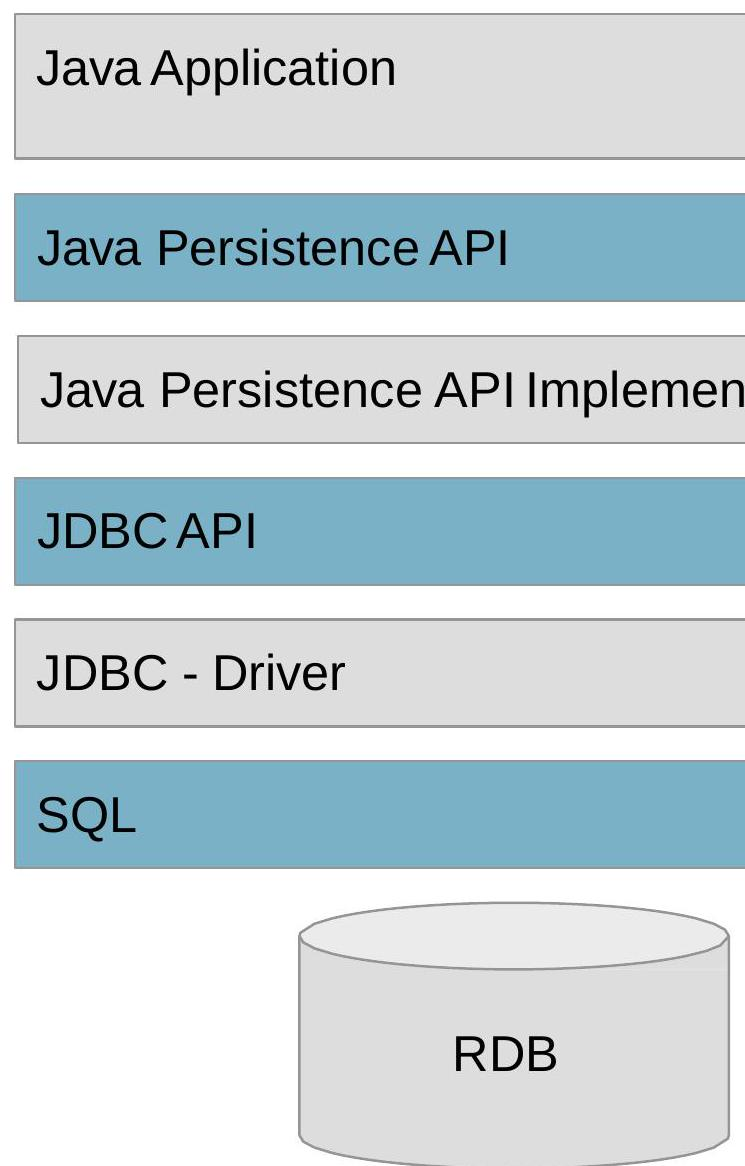
\includegraphics[width=0.8\linewidth]{images/2025_01_02_5ba1dc702e9f94ba8e06g-29.jpg}
\end{minipage}
\end{concept}

\begin{KR}{JPA Entity Erstellung}
\begin{enumerate}
    \item Entity-Klasse definieren:
    \begin{itemize}
        \item @Entity Annotation
        \item ID-Feld mit @Id markieren
    \end{itemize}
    \item Beziehungen definieren:
    \begin{itemize}
        \item @OneToMany, @ManyToOne etc.
        \item Navigationsrichtung festlegen
    \end{itemize}
    \item Validierung hinzufügen:
    \begin{itemize}
        \item @NotNull, @Size etc.
        \item Geschäftsregeln
    \end{itemize}
\end{enumerate}
\end{KR}

\begin{KR}{JPA Entity Design}

\textbf{1. Grundstruktur}

\begin{minipage}[t]{0.5\textwidth}
\begin{itemize}
    \item \textbf{Basisanforderungen:}
    \begin{itemize}
        \item Default Constructor
        \item Serializable (optional)
        \item Getter/Setter
    \end{itemize}
    \end{itemize}
\end{minipage}
\begin{minipage}[t]{0.5\textwidth}
\begin{itemize}
    \item \textbf{Identifikation:}
    \begin{itemize}
        \item Primary Key Strategie
        \item Natural vs. Surrogate Key
    \end{itemize}
\end{itemize}
\end{minipage}
\vspace{1mm}\\
\textbf{2. Beziehungen}

\begin{minipage}[t]{0.5\textwidth}
\begin{itemize}
    \item \textbf{Kardinalität:}
    \begin{itemize}
        \item OneToOne
        \item OneToMany/ManyToOne
        \item ManyToMany
    \end{itemize}
\end{itemize}
\end{minipage}
\begin{minipage}[t]{0.5\textwidth}
\begin{itemize}
    \item \textbf{Richtung:}
    \begin{itemize}
        \item Unidirektional
        \item Bidirektional
    \end{itemize}
    \item \textbf{Lifecycle:}
    \begin{itemize}
        \item Cascade-Operationen
        \item Orphan Removal
    \end{itemize}
\end{itemize}
\end{minipage}

\textbf{3. Optimierungen}

\begin{minipage}[t]{0.5\textwidth}
\begin{itemize}
    \item \textbf{Lazy Loading:}
    \begin{itemize}
        \item Fetch-Strategien
        \item Join Fetching
    \end{itemize}
\end{itemize}
\end{minipage}
\begin{minipage}[t]{0.5\textwidth}
\begin{itemize}
    \item \textbf{Caching:}
    \begin{itemize}
        \item First-Level Cache
        \item Second-Level Cache
    \end{itemize}
\end{itemize}
\end{minipage}
\end{KR}


\subsection{Design Patterns für Persistenz}

\begin{theorem}{Persistenz Design Patterns}\\
Drei grundlegende Ansätze für die Persistenzschicht:
\begin{itemize}
    \item \textbf{Active Record (Anti-Pattern):}
    \begin{itemize}
        \item Jede Entität verwaltet eigene Persistenz
        \item Vermischung von Fachlichkeit und Technik in einer Klasse
        \item Wrapper für Datenbankzeilen, spiegelt DB-Struktur direkt
        \item Schlechte Testbarkeit der Domänenlogik
        \item Schlechte Wartbarkeit und Erweiterbarkeit
    \end{itemize}
    \item \textbf{Data Access Object (DAO):}
    \begin{itemize}
        \item Kapselung des Datenbankzugriffs
        \item Trennung von Fachlichkeit und Technik
        \item Domänenklasse hat hohe Kohäsion
        \item Gute Testbarkeit durch Mocking
        \item Bevorzugtes Design ohne O/R-Mapper
    \end{itemize}
    \item \textbf{Repository (DDD):}
    \begin{itemize}
        \item Abstraktionsschicht über Data-Mapper
        \item Zentralisierung von Datenbankabfragen
        \item Komplexere Implementierung, aber Unterstützung für Komplexere Abfragen
        \item Domänenorientierte Schnittstelle
        \item Häufig in Kombination mit Spring Data
    \end{itemize}
\end{itemize}
\end{theorem}

\begin{remark}
    Spring Data unterstützt die automatische Generierung von Repository-Implementierungen basierend auf Methodennamen. Dies reduziert den Implementierungsaufwand erheblich.
\end{remark}

\begin{KR}{Analyse der Persistenzanforderungen}

    \begin{minipage}[t]{0.5\textwidth}
\textbf{1. Funktionale Anforderungen}
\begin{itemize}
    \item Datenmodell und Beziehungen
    \item Abfrageanforderungen
    \item Transaktionsverhalten 
\end{itemize}

\textbf{2. Nicht-funktionale\\ Anforderungen}
\begin{itemize}
    \item Performance
    \item Skalierbarkeit
    \item Wartbarkeit
    \item Konsistenz
\end{itemize}
\end{minipage}
\begin{minipage}[t]{0.5\textwidth}
\textbf{3. Technische Randbedingungen}
\begin{itemize}
    \item Vorhandene Systeme
    \item Datenbanktyp
    \item Entwicklungsumgebung
\end{itemize}

\textbf{4. Designentscheidungen}
\begin{itemize}
    \item Persistenzstrategie wählen
    \item Framework-Auswahl
    \item Architekturmuster festlegen
\end{itemize}
\end{minipage}
\end{KR}

\begin{concept}{Common Pitfalls in Persistence Implementation}
\paragraph{1. JPA Fallstricke}

    \textbf{N+1 Problem:}
    \begin{itemize}
        \item Symptom: Für jedes Objekt wird eine zusätzliche Query ausgeführt
        \item Lösung: Join Fetch oder Eager Loading strategisch einsetzen
    \end{itemize}
     \textbf{LazyInitializationException:}
    \begin{itemize}
        \item Symptom: Zugriff auf lazy geladene Referenz außerhalb der Session
        \item Lösung: Transaktionen richtig abgrenzen oder Fetch Join verwenden
    \end{itemize}
     \textbf{Bidirektionale Beziehungen:}
    \begin{itemize}
        \item Symptom: Inkonsistente Objektzustände
        \item Lösung: Helper-Methoden für Beziehungspflege
    \end{itemize}


\paragraph{2. Performance Probleme}
     \textbf{Zu viele Queries:}
    \begin{itemize}
        \item Problem: Ineffiziente Datenbankzugriffe
        \item Lösung: Batch Processing, Bulk Operations
    \end{itemize}
     \textbf{Memory Leaks:}
    \begin{itemize}
        \item Problem: Große Result Sets
        \item Lösung: Pagination, Streaming Results
    \end{itemize}
\end{concept}

\begin{KR}{Persistenzstrategie wählen}\\
\textbf{1. Anforderungen analysieren}
\begin{itemize}
    \item \textbf{Funktional:}
    \begin{itemize}
        \item Datenmodell-Komplexität
        \item Abfrageanforderungen
        \item Transaktionsverhalten
    \end{itemize}
    \item \textbf{Nicht-funktional:}
    \begin{itemize}
        \item Performance
        \item Skalierbarkeit
        \item Wartbarkeit
    \end{itemize}
\end{itemize}

\textbf{2. Technologien evaluieren}
\begin{itemize}
    \item \textbf{JDBC:}
    \begin{itemize}
        \item Direkte Kontrolle
        \item Hohe Performance
        \item Hoher Implementierungsaufwand
    \end{itemize}
    \item \textbf{JPA:}
    \begin{itemize}
        \item Standardisiert
        \item Produktiv
        \item Lernkurve
    \end{itemize}
    \item \textbf{NoSQL:}
    \begin{itemize}
        \item Flexibles Schema
        \item Hohe Skalierbarkeit
        \item Spezielle Anwendungsfälle
    \end{itemize}
\end{itemize}
\end{KR}

\begin{example2}{Prüfungsaufgabe: Design Pattern Vergleich}\\
\textbf{Aufgabe:}
Vergleichen Sie Active Record, DAO und Repository Pattern.

\textbf{Analysematrix:}
\begin{itemize}
    \item \textbf{Active Record:}
    \begin{itemize}
        \item \textbf{Vorteile:}
        \begin{itemize}
            \item Einfache Implementierung
            \item Schnell zu entwickeln
        \end{itemize}
        \item \textbf{Nachteile:}
        \begin{itemize}
            \item Keine Trennung der Belange
            \item Schlechte Testbarkeit
            \item Vermischung von Fachlogik und Persistenz
        \end{itemize}
    \end{itemize}
    
    \item \textbf{DAO:}
    \begin{itemize}
        \item \textbf{Vorteile:}
        \begin{itemize}
            \item Klare Trennung der Belange
            \item Gute Testbarkeit
            \item Austauschbare Implementierung
        \end{itemize}
        \item \textbf{Nachteile:}
        \begin{itemize}
            \item Mehr Initialaufwand
            \item Zusätzliche Abstraktionsebene
        \end{itemize}
    \end{itemize}
    
    \item \textbf{Repository:}
    \begin{itemize}
        \item \textbf{Vorteile:}
        \begin{itemize}
            \item Domänenorientierte Schnittstelle
            \item Zentrale Abfragelogik
            \item DDD-konform
        \end{itemize}
        \item \textbf{Nachteile:}
        \begin{itemize}
            \item Komplexere Implementierung
            \item Höhere Lernkurve
        \end{itemize}
    \end{itemize}
\end{itemize}
\end{example2}

\subsubsection{Implementation der Patterns}

\begin{KR}{DAO Implementation}\\
Schritte zur Implementierung eines DAOs:
\begin{enumerate}
    \item Interface definieren:
    \begin{itemize}
        \item CRUD-Methoden (Create, Read, Update, Delete)
        \item Spezifische Suchmethoden
    \end{itemize}
    \item Domänenklasse erstellen:
    \begin{itemize}
        \item Nur fachliche Attribute
        \item Keine Persistenzlogik
    \end{itemize}
    \item DAO-Implementierung:
    \begin{itemize}
        \item Datenbankzugriff kapseln
        \item O/R-Mapping implementieren
        \item Transaktionshandling
    \end{itemize}
\end{enumerate}
\end{KR}



\begin{concept}{DAO Pattern mit JDBC}\\
    \textbf{Implementierungsstruktur:}

    \begin{minipage}[t]{0.5\textwidth}
\begin{itemize}
    \item \textbf{Interface:}
    \begin{itemize}
        \item Definiert CRUD-Operationen
        \item Definiert spezifische \\ Abfragen
    \end{itemize}
    \item \textbf{Domänenklasse:}
    \begin{itemize}
        \item Reine Geschäftslogik
        \item Keine Persistenzlogik
    \end{itemize}
\end{itemize}
\end{minipage}
\begin{minipage}[t]{0.5\textwidth}
    \begin{itemize}
    \item \textbf{Implementierung:}
    \begin{itemize}
        \item Verwendet JDBC für\\ DB-Zugriff
        \item Implementiert O/R-Mapping
        \item Behandelt Fehler
    \end{itemize}
\end{itemize}
\end{minipage}
\end{concept}

\begin{example2}{DAO Implementation}
\textbf{1. Interface definieren:}
\begin{lstlisting}[language=Java, style=basesmol]
public interface UserDAO {
    void insert(User user);
    User findById(long id);
    List<User> findAll();
    void update(User user);
    void delete(User user);
}
\end{lstlisting}

\textbf{2. JDBC-Implementierung:}
\begin{lstlisting}[language=Java, style=basesmol]
public class JdbcUserDAO implements UserDAO {
    private Connection getConnection() {
        // Verbindungsaufbau
    }
    public User findById(long id) {
        Connection conn = getConnection();
        try {
            PreparedStatement ps = conn.prepareStatement(
                "SELECT * FROM users WHERE id = ?");
            ps.setLong(1, id);
            ResultSet rs = ps.executeQuery();
            if (rs.next()) {
                return mapUser(rs);
            }
            return null;
        } finally {
            conn.close();
        }
    }
    private User mapUser(ResultSet rs) {
        User user = new User();
        user.setId(rs.getLong("id"));
        user.setName(rs.getString("name"));
        return user;
    }
}
\end{lstlisting}
\end{example2}



\begin{example2}{Typische Prüfungsaufgabe: Parent-Child Beziehung}\\
\textbf{Szenario:}
Implementieren Sie eine bidirektionale One-to-Many Beziehung zwischen Department und Employee.

\textbf{1. Entity-Klassen:}
\begin{lstlisting}[language=Java, style=basesmol]
@Entity
public class Department {
    @Id @GeneratedValue
    private Long id;
    private String name;
    
    @OneToMany(mappedBy = "department", 
               cascade = CascadeType.ALL,
               orphanRemoval = true)
    private List<Employee> employees = new ArrayList<>();
    
    // Helper Methoden
    public void addEmployee(Employee employee) {
        employees.add(employee);
        employee.setDepartment(this);
    }
    
    public void removeEmployee(Employee employee) {
        employees.remove(employee);
        employee.setDepartment(null);
    }
}

@Entity
public class Employee {
    @Id @GeneratedValue
    private Long id;
    
    @ManyToOne(fetch = FetchType.LAZY)
    @JoinColumn(name = "department_id")
    private Department department;
}
\end{lstlisting}

\textbf{2. Repository Interface:}
\begin{lstlisting}[language=Java, style=basesmol]
public interface DepartmentRepository 
    extends JpaRepository<Department, Long> {
    
    @Query("SELECT d FROM Department d " +
           "LEFT JOIN FETCH d.employees " +
           "WHERE d.id = :id")
    Optional<Department> findByIdWithEmployees(
        @Param("id") Long id);
}
\end{lstlisting}

\textbf{3. Service Layer:}
\begin{lstlisting}[language=Java, style=basesmol]
@Service
@Transactional
public class DepartmentService {
    @Autowired
    private DepartmentRepository repository;
    
    public void addEmployeeToDepartment(
            Long deptId, Employee employee) {
        Department dept = repository
            .findById(deptId)
            .orElseThrow(() -> 
                new EntityNotFoundException());
        dept.addEmployee(employee);
        repository.save(dept);
    }
}
\end{lstlisting}
\end{example2}



\begin{example2}{Praktische Implementierungsbeispiele}\\
\textbf{1. Optimistisches Locking:}
\begin{lstlisting}[language=Java, style=basesmol]
@Entity
public class Account {
    @Version
    private Long version;
    
    private BigDecimal balance;
    
    public void withdraw(BigDecimal amount) {
        if (balance.compareTo(amount) < 0) {
            throw new InsufficientFundsException();
        }
        balance = balance.subtract(amount);
    }
}
\end{lstlisting}

\textbf{2. Entity Lifecycle Callbacks:}
\begin{lstlisting}[language=Java, style=basesmol]
@Entity
public class AuditedEntity {
    @PrePersist
    void onCreate() {
        this.createdDate = LocalDateTime.now();
    }
    
    @PreUpdate
    void onUpdate() {
        this.lastModified = LocalDateTime.now();
    }
}
\end{lstlisting}

\textbf{3. Custom Repository Implementation:}
\begin{lstlisting}[language=Java, style=basesmol]
@Repository
public class CustomOrderRepositoryImpl 
    implements CustomOrderRepository {
    
    @PersistenceContext
    private EntityManager em;
    
    public List<Order> findComplexOrders(
            OrderCriteria criteria) {
        CriteriaBuilder cb = em.getCriteriaBuilder();
        CriteriaQuery<Order> query = 
            cb.createQuery(Order.class);
        Root<Order> root = query.from(Order.class);
        
        // Complex criteria building
        Predicate[] predicates = buildPredicates(
            cb, root, criteria);
        query.where(predicates);
        
        return em.createQuery(query)
                 .getResultList();
    }
}
\end{lstlisting}
\end{example2}


